\documentclass[review]{elsarticle}
% Target journal: Vehicular Communications (Elsevier). Review option = double spaced.
% Compile: pdflatex main.tex
% NUMBER POLICY: every number in this file traces to a results JSON in
%   ../results/ (attack_results_merged.json, train_report.json).
%   Claims not yet backed by a committed artifact are marked [FULL PROTOCOL
%   PENDING] and MUST NOT be unmarked before the run exists. See CLAIMS.md.

\usepackage{amsmath,amssymb}
\usepackage{graphicx}
\usepackage{booktabs}
\usepackage{url}
\usepackage{multirow}
\usepackage{tikz}
\usetikzlibrary{arrows.meta, positioning}

% Marker for claims that await the full-scale protocol runs (3 seeds,
% PGD-50, extended grid, defenses). Greppable: never remove a \FULLP marker
% until the backing result JSON exists in ../results/.
\newcommand{\FULLP}[1]{[\emph{#1 --- full-protocol run pending}]}

\journal{Vehicular Communications}

\begin{document}

\begin{frontmatter}

\title{The Price of Compliance: Emission-Mask-Constrained Adversarial Attacks
on Deep Learning Spectrum Sensing in the 5.9\,GHz ITS Band}

\author[inst1]{Parveen Dhankhar\corref{cor1}}
\ead{parveendhankhar2005@gmail.com}
\author[inst1]{Davesh Vats}
\ead{vatsdavesh@gmail.com}

\cortext[cor1]{Corresponding author.}
\affiliation[inst1]{organization={Department of Computer Science and Engineering,
Vaish College of Engineering, Rohtak, India},
            city={Rohtak},
            country={India}}

\begin{abstract}
Deep learning (DL) classifiers are increasingly proposed for spectrum sensing
in Vehicle-to-Everything (V2X) networks, and are known to be vulnerable to
adversarial perturbations. Prior wireless adversarial-ML evaluations, however,
either perturb receiver-side features directly---a threat no radio transmitter
can realize---or transmit without regard for spectrum rules. This paper
formalizes and quantifies the attacker that actually exists in the 5.9\,GHz ITS
band: a \emph{compliant attacker} that respects its regulatory allocation and
emission mask while optimizing a waveform-domain perturbation end-to-end
through the attacker-to-receiver channel and the receiver's STFT front-end. We
instantiate the threat model on a post-FCC coexistence sensing task in a
20\,MHz window straddling the 5895\,MHz boundary: C-V2X PC5 and legacy
IEEE~802.11p are co-channel in the ITS band (the transition-period problem),
with U-NII-4 Wi-Fi below the boundary. On TR~37.885-inspired urban, highway,
and rural channels, an unconstrained (``genie'') attacker reaches 20\% conditional attack
success at $-44$\,dB relative received power, while the mask-compliant attacker
needs $-37$ to $-39$\,dB: an \emph{emission-mask price of compliance of
5--7\,dB} (untargeted) and 16--18\,dB for targeted ``cloaking'' of an active
transmitter as noise. The absolute regime is the more alarming finding: an
\emph{undefended} sensing CNN is broken by a rule-abiding transmitter operating
tens of dB below the victim signal level (96.7\% conditional ASR at
$-10$\,dB). We also translate the legacy feature-space threat model into
physical power, showing that receiver-internal $\epsilon$-balls describe a
perturbation that mostly cannot survive its own physical realization, while
a purpose-optimized waveform at the same implied power is far stronger. As the matched defense, mask-matched adversarial training shifts
the compliant-attacker threshold by $+14$\,dB (doubling the price of
compliance) at no clean-accuracy cost, with robustness honestly bounded by
its training power range. We propose Minimum Effective Attack Power (MEAP) and
Price-of-Compliance (PoC) as physically grounded, transferable security
metrics, and release the complete framework (waveform generators, channels,
attack, defenses, checkpoints, result JSONs with embedded seeds and
configurations) for reproduction.
\end{abstract}

\begin{keyword}
V2X \sep spectrum sensing \sep adversarial machine learning \sep 5.9 GHz
\sep C-V2X \sep IEEE 802.11p \sep emission mask \sep physical-layer security
\end{keyword}

\end{frontmatter}

% ============================================================================
\section{Introduction}
\label{sec:intro}

The 5.9\,GHz ITS band is in the middle of the most consequential spectrum
decision of its history. In FCC~20-164 (2020), the Commission reallocated the
band: the upper 30\,MHz (5895--5925\,MHz) is dedicated to C-V2X, while the
lower 45\,MHz (5850--5895\,MHz) was opened to unlicensed U-NII-4
operation~\cite{fcc2020}; the 2024 Second Report and Order completed the
transition rules and set the DSRC sunset in motion~\cite{fcc2024}. During and
after this transition, coexistence sensing---determining \emph{which}
technology is transmitting, not merely whether energy is present---becomes a
safety-relevant function: roadside units and vehicles must distinguish C-V2X
PC5, legacy 802.11p still on the road, and unlicensed Wi-Fi spilling up to the
boundary. Deep learning classifiers are the natural candidate for this
four-way technology recognition, following their success in wireless signal
classification~\cite{o2018,girmay2023}.

The same classifiers, however, inherit the adversarial fragility of deep
networks. A large literature demonstrates that wireless DL classifiers can be
fooled by small, deliberate perturbations~\cite{sadeghi2019,liu2022}. Yet the
threat models in that literature have a physical gap. Feature-space attacks
edit the receiver's input (IQ frames or spectrograms) directly---an adversary
with that access does not need adversarial examples at all. Over-the-air and
channel-aware attacks~\cite{kim2020,sagduyu2021,radioshock2026} closed part of
the gap by transmitting real waveforms through modeled channels, and recent
work has targeted wideband spectrum sensing directly~\cite{zheng2026}. But
none of these asks the question that every real attacker in the 5.9\,GHz band
must answer: \emph{the attacker must obey the very spectrum rules it is
attacking}. A C-V2X device may only transmit in its 10\,MHz ITS allocation
under an emission mask (ETSI EN~302~571~\cite{etsi302571} in Europe; FCC rules
in the US); a U-NII-4 device must stay below 5895\,MHz. An attack that
requires illegal emissions is not an attack on the system---it is a
regulatory violation that conventional spectrum enforcement already handles.

This paper therefore poses and quantifies the \emph{compliant-attacker}
threat model: a spectrum-rule-abiding adversary that transmits only within its
allocation, under an emission mask, with bounded power, while optimizing its
waveform end-to-end through the physical channel and the receiver's
front-end. The question that determines whether mask compliance is itself a
defense is quantitative: \emph{how much attack power does compliance cost?}
We answer it with two new metrics---Minimum Effective Attack Power (MEAP) and
Price of Compliance (PoC)---and with a fully differentiable
waveform$\to$channel$\to$STFT$\to$CNN attack chain whose perturbations are
projected, at every optimization step, onto the physically feasible set.

Our contributions are:
\begin{enumerate}
  \item \textbf{Threat model.} The compliant attacker: an emission-mask and
  allocation constraint on waveform-domain adversarial perturbations, to our
  knowledge the first such constraint in the wireless adversarial-ML
  literature (Table~\ref{tab:threat}).
  \item \textbf{Task.} A post-FCC coexistence sensing benchmark in a
  20\,MHz window straddling the 5895\,MHz boundary: block-exact 802.11p and
  U-NII-4 generators and a rate-matched C-V2X PC5 generator, co-channel
  802.11p/PC5 in the ITS allocation (the transition problem), with an
  honest energy-feature baseline showing where deep learning is and is not
  needed.
  \item \textbf{Attack.} A differentiable projected-gradient attack over the
  waveform, with out-of-band nulling, an in-band PSD cap, and an explicit
  power budget defined as the physical attack-to-signal power ratio (PSR).
  \item \textbf{Metrics.} MEAP and PoC: power-domain, attacker-agnostic
  robustness measures suitable for certification-style reporting.
  \item \textbf{Findings.} On TR~37.885-inspired channels: compliance costs
  the attacker ${\sim}5$--7\,dB (untargeted) and 16--18\,dB (targeted
  cloaking); an undefended CNN is nevertheless broken by a compliant attacker
  at deeply negative PSR; the legacy feature-space $\epsilon$-ball assumes a
  hidden power budget we make measurable; and mask-matched adversarial
  training shifts the compliant-attacker threshold by $+14$\,dB at no
  clean-accuracy cost. Compliance \emph{delays} the attack; so does the
  defense; neither prevents it.
\end{enumerate}

\paragraph{Scope and honesty} All attack numbers in this paper are
prototype-scale (one training seed, two attack seeds, 300 evaluation windows,
PGD-10) and are labeled as such; the full protocol (3 seeds, PGD-50, extended
grid, rural scenario) is specified in the released repository; rural,
PGD-50, a second attack seed, the mask-cap sensitivity, the defense study,
and the feature-space comparison are included here, and
\FULLP{the 3-seed training protocol completes the statistics}. Every number
traces to a result JSON with embedded configuration. The undefended model is
the subject of Sections~\ref{sec:poc}--\ref{sec:featurespace}; the defense
study (Section~\ref{sec:defenses}) quantifies how much of the threat
adversarial training removes.

\section{Related Work and Threat-Model Positioning}
\label{sec:related}

\paragraph{DL spectrum sensing and ITS-band recognition} Deep learning radio
signal classification was established at scale by O'Shea et
al.~\cite{o2018}. For the ITS band specifically, Girmay et
al.~\cite{girmay2023} built CNN-based technology recognition and traffic
characterization for coexisting wireless technologies---the coexistence
problem our task generator mirrors. These works establish capability, not
robustness.

\paragraph{Adversarial attacks on wireless DL} Sadeghi and
Larsson~\cite{sadeghi2019} demonstrated white-box attacks on modulation
classifiers in feature space. Liu et al.~\cite{liu2022} attacked
spectrum sensing in cognitive-radio IoT, again at the feature level.
Over-the-air reality was first confronted by Kim et al.~\cite{kim2020} and
matured into channel-aware attacks~\cite{sagduyu2021}, which optimize the
transmit waveform through a modeled channel; RadioShock~\cite{radioshock2026}
demonstrated OTA attacks with channel-state estimation, and Zheng et
al.~\cite{zheng2026} brought targeted attacks to wideband spectrum sensing.
Defense-side, Zhao et al.~\cite{zhao2024} proposed statistical detection of
adversarial spectrum attacks, and Croce and Hein~\cite{croce2020} established
reliable attack ensembles for robustness evaluation. In the standards world,
Habler et al.~\cite{habler2025} mapped adversarial-ML threats onto O-RAN
architectures---the deployment context our metrics target.

\paragraph{Positioning} Table~\ref{tab:threat} positions the compliant
attacker. The differentiator is not ``channel awareness'' (present
in~\cite{sagduyu2021,radioshock2026}) nor the sensing task
(present in~\cite{liu2022,zheng2026}); it is the \emph{regulatory constraint
set}: allocation, emission mask, and an explicit power budget swept as the
independent variable. To our knowledge no prior work constrains a wireless
adversary to its spectrum rules, and none reports a power-domain
price-of-compliance analysis. This matters because compliance is the one
attacker property that is \emph{verifiable by regulators}: an attacker that
must obey the mask is within the reach of conformance testing, which makes
the resulting robustness metrics deployable (Section~\ref{sec:standards}).

\begin{table}[t]
\centering
\caption{Threat-model comparison. ``Mask'' = regulatory allocation +
emission-mask constraint on the transmitted adversarial perturbation.}
\label{tab:threat}
\small
\begin{tabular}{lccccc}
\toprule
Work & Waveform & Channel & Mask & Power sweep & Task \\
\midrule
Sadeghi \& Larsson~\cite{sadeghi2019} & -- & -- & -- & -- & modulation \\
Liu et al.~\cite{liu2022} & -- & -- & -- & -- & spectrum sensing \\
Kim et al.~\cite{kim2020} & \checkmark & \checkmark & -- & fixed & modulation \\
Kim et al.~\cite{sagduyu2021} & \checkmark & \checkmark & -- & fixed & modulation \\
Zheng et al.~\cite{zheng2026} & \checkmark & \checkmark & -- & fixed & wideband sensing \\
RadioShock~\cite{radioshock2026} & \checkmark & \checkmark & -- & fixed & communication \\
\textbf{This work} & \checkmark & \checkmark & \textbf{\checkmark} & \textbf{MEAP} & \textbf{ITS coexistence} \\
\bottomrule
\end{tabular}
\end{table}

\section{System Model}
\label{sec:system}

\subsection{Post-FCC coexistence sensing task}
\label{sec:task}

The sensing receiver observes a 20\,MHz complex-baseband window
(2048 samples at $F_S = 20$\,MHz, i.e., 102.4\,\textmu s) centered on the
5895\,MHz boundary, covering 5885--5905\,MHz (Fig.~\ref{fig:bandplan}). This
boundary-straddling placement is the physically interesting vantage point:
the upper half contains the ITS allocation (5895--5905\,MHz is the lowest
C-V2X channel), the lower half the upper edge of U-NII-4 unlicensed
operation. The classification task is four-way (Table~\ref{tab:bandplan}):

\begin{figure}[t]
\centering
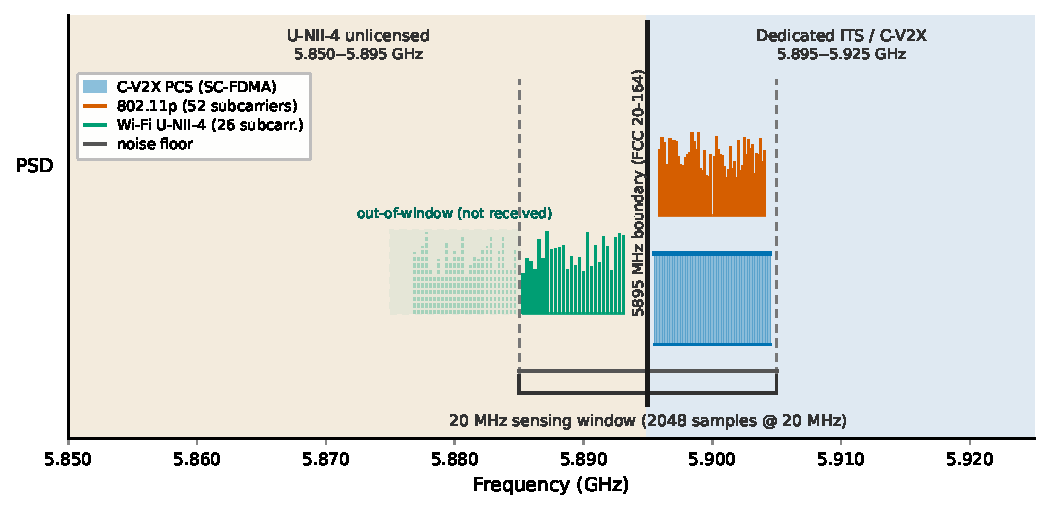
\includegraphics[width=0.98\linewidth]{figs/band_plan.pdf}
\caption{Post-FCC 5.9\,GHz band plan as seen by the boundary-straddling
sensing window (stylized PSD, not to scale). Shading marks the two
regulatory blocks created by FCC~20-164: unlicensed U-NII-4 below the
5895\,MHz boundary and the dedicated ITS/C-V2X allocation above it. C-V2X
PC5 (flat-topped SC-FDMA block) and IEEE~802.11p (52 raised subcarrier
stems) are deliberately co-channel in the lowest 10\,MHz ITS channel; the
Wi-Fi class is the partial 26-subcarrier view of a U-NII-4 channel centered
10\,MHz below the window, whose out-of-window half (dashed ghost) is removed
by the receiver's anti-alias filter.}
\label{fig:bandplan}
\end{figure}

\begin{table}[h]
\centering
\caption{Post-FCC band plan as seen by the sensing window (frequencies
relative to the 5895\,MHz boundary). PC5 and 802.11p are deliberately
co-channel: the transition-period coexistence problem.}
\label{tab:bandplan}
\small
\begin{tabular}{llll}
\toprule
Class & Standard basis & Occupied (MHz) & Generation \\
\midrule
C-V2X PC5 & Rel-14 SC-FDMA$^{\dagger}$ & $[+0.5, +9.5]$ & contiguous DFT-s-OFDM \\
802.11p & 802.11-2012 OFDM & $[+0.94, +9.06]$ & 52-sub IFFT+CP, DC nulled \\
Wi-Fi U-NII-4 & 802.11 20\,MHz OFDM & $[-9.69, -1.88]$ & 26 in-window subcarr. \\
Noise & -- & full band & complex AWGN \\
\bottomrule
\multicolumn{4}{l}{\footnotesize $^{\dagger}$rate-matched stylization: 450$\times$20\,kHz
(9\,MHz = Rel-14 occupied BW); SCS/DMRS not modeled (Sec.~\ref{sec:limitations}).}
\end{tabular}
\end{table}

Two design decisions deserve justification. First, \emph{802.11p and PC5 are
co-channel} in the ITS allocation: during the multi-year DSRC sunset,
roadside infrastructure must classify both technologies sharing the same
spectrum, and region-energy features provably cannot separate them---our
logistic-regression baseline on region-energy and envelope features reaches
only 77.75\% on this pair, while the CNN reaches 100\% (four-class baseline:
88.62\% vs 100\%). The DL-necessity claim is thus confined to what physics
cannot do, unlike prior work where classes are region-separable and
``deep learning needed'' claims do not survive an energy baseline. Second,
\emph{Wi-Fi is region-separable from the ITS pair} (it lives below the
boundary); this is correct post-FCC physics, and we state it rather than
engineer it away.

The waveform generators are block-exact where the standards allow it at
$F_S=20$\,MHz: 802.11p~\cite{ieee80211} uses 52 subcarriers at 156.25\,kHz spacing with a
1.6\,\textmu s cyclic prefix and a nulled DC subcarrier; the U-NII-4 class is
the physically correct partial view of a 20\,MHz 802.11 channel (312.5\,kHz
spacing, 0.8\,\textmu s guard interval) whose center lies 10\,MHz below the
window---only the 26 in-window subcarriers are generated, as the receiver's
anti-alias filter removes the rest. PC5 is a rate-matched stylization of
Rel-14~\cite{ts36211}: 450 subcarriers at 20\,kHz (the same 9\,MHz occupied
bandwidth as 50 PRBs at 15\,kHz), chosen so the block is an exact integer at
$F_S=20$\,MHz; single-carrier structure and PAPR are preserved (measured:
6.1\,dB PC5 vs 8.8/8.6\,dB for the OFDM classes). All data symbols are
QPSK; pilots and preambles are not modeled.

\subsection{Channel model}
\label{sec:channels}

Channels are simplified, TR~37.885-inspired~\cite{tr37885} block-fading
tapped-delay models: highway (120\,km/h, Rician $K=10$\,dB first tap, 5
taps, ${\sim}$0.4\,\textmu s spread), urban (50\,km/h, Rayleigh, 6 taps,
${\sim}$1.3\,\textmu s spread, UMa-flavored), and rural (30\,km/h, $K=5$\,dB,
3 taps). Block fading is justified even at highway speed: the maximum Doppler
(${\sim}$656\,Hz at 5.9\,GHz) gives a decorrelation time of
${\sim}$0.55--0.76\,ms, far exceeding the 102.4\,\textmu s window. The
victim link and the attacker-to-receiver link draw independent channel
realizations. Deviations from the spec's CDL profiles (first-tap-only
Rician, UMa-flavored urban spread) are disclosed in
Section~\ref{sec:limitations}.

\subsection{Receiver front-end and classifier}
\label{sec:frontend}

The receiver computes a complex STFT (256-point, 128 hop, Hann window,
two-sided and frequency-shifted) yielding $256\times15$ frames, from which
two streams are derived: log-magnitude (z-scored, clamped) and the per-bin
temporal phase difference (a phase-vocoder-style frequency-offset estimate).
Both streams feed a dual-stream Inception-Time CNN (86,052 parameters),
carried over from our prior work~\cite{dhankhar2026} for architectural
comparability; a magnitude-only variant (40,980 parameters) serves as the
pre-registered stream ablation. The entire chain is implemented in PyTorch
and is differentiable end-to-end from time-domain waveform to logits---the
enabler of the waveform-domain attack. Training uses the prior work's recipe
(label smoothing 0.1, TF-CutMix, Gaussian augmentation, Adam 5e-4, cosine
schedule) on 3,200 training windows (800 held-out validation windows) with
mixed scenarios and SNR drawn uniformly from [5,~25]\,dB.

\section{The Compliant Attacker}
\label{sec:attack}

\begin{figure}[t]
\centering
\resizebox{\textwidth}{!}{%
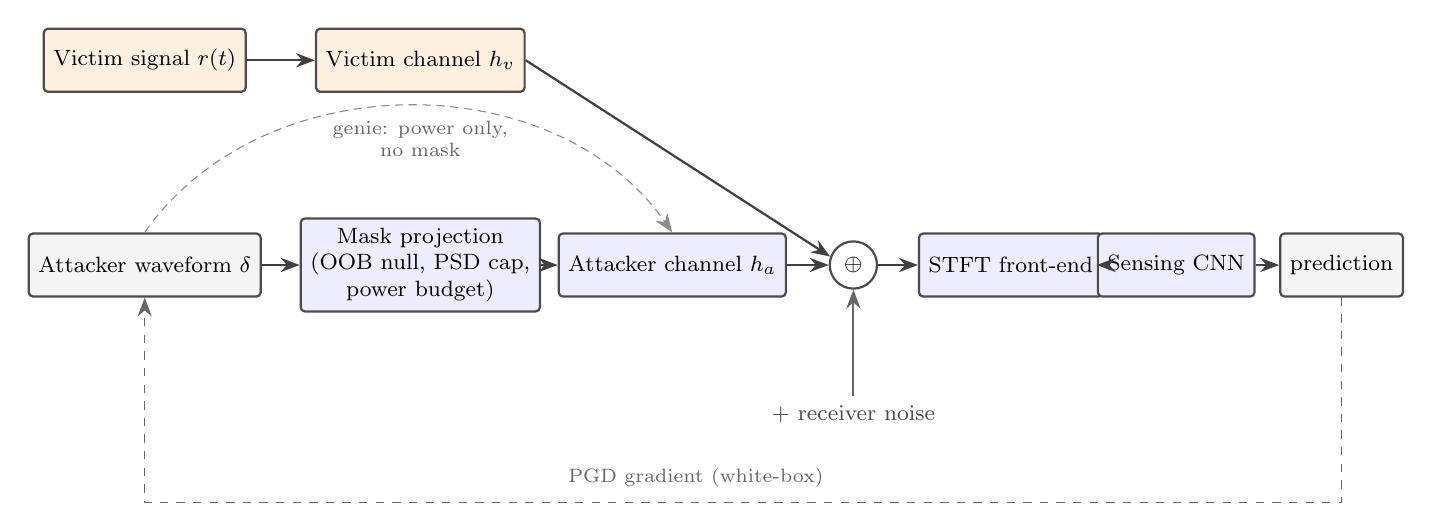
\begin{tikzpicture}[
  font=\footnotesize,
  box/.style={draw=black!70, thick, rounded corners=1.5pt, align=center,
              inner sep=3.5pt, minimum height=8mm},
  io/.style={box, fill=black!4},
  atk/.style={box, fill=blue!7},
  vic/.style={box, fill=orange!12},
  arr/.style={-{Stealth[length=2.4mm]}, thick, black!75},
  fb/.style={-{Stealth[length=2.4mm]}, dashed, black!60},
  gen/.style={-{Stealth[length=2.4mm]}, densely dashed, black!45},
]
% attacker chain (middle row)
\node[io] (delta) at (0,0) {Attacker waveform $\delta$};
\node[atk] (mask) at (3.5,0) {Mask projection\\(OOB null, PSD cap,\\power budget)};
\node[atk] (ha) at (6.7,0) {Attacker channel $h_a$};
\node[circle, draw=black!70, thick, minimum size=6mm, inner sep=0pt]
  (sum) at (9.0,0) {$\oplus$};
\node[atk] (stft) at (11.0,0) {STFT front-end};
\node[atk] (cnn) at (13.1,0) {Sensing CNN};
\node[io] (pred) at (15.2,0) {prediction};
% victim path (top row) joins the same junction
\node[vic] (victim) at (0,2.6) {Victim signal $r(t)$};
\node[vic] (hv) at (3.5,2.6) {Victim channel $h_v$};
% receiver noise into the junction
\node[black!70] (noise) at (9.0,-1.9) {$+$ receiver noise};
% arrows: attacker chain
\draw[arr] (delta) -- (mask);
\draw[arr] (mask) -- (ha);
\draw[arr] (ha) -- (sum);
\draw[arr] (sum) -- (stft);
\draw[arr] (stft) -- (cnn);
\draw[arr] (cnn) -- (pred);
\draw[arr] (victim) -- (hv);
\draw[arr] (hv.east) -- (sum.160);
\draw[arr, black!60] (noise) -- (sum.270);
% genie bypass: power only, no mask
\draw[gen] (delta.north) to[out=55,in=125] (ha.north);
\node[black!60, align=center, font=\scriptsize] at (3.5,1.6)
  {genie: power only,\\no mask};
% PGD feedback (white-box)
\draw[fb] (pred.south) -- ++(0,-2.6) -| (delta.south);
\node[black!60, anchor=south, font=\scriptsize] at (7.0,-2.95)
  {PGD gradient (white-box)};
\end{tikzpicture}%
}
\caption{Threat model of the compliant attacker. The attacker optimizes a
waveform-domain perturbation $\delta$ end-to-end through its own channel
$h_a$, the receiver's STFT front-end, and the sensing CNN; the dashed
return path carries the white-box PGD gradient. The \emph{compliant}
variant projects $\delta$ onto the feasible set (out-of-band null, in-band
PSD cap, transmit-power budget) at every optimization step, while the
\emph{genie} variant bypasses the mask projection and obeys only the power
budget. The victim signal $r(t)$ arrives through an independent channel
$h_v$; the junction also adds receiver noise.}
\label{fig:threat}
\end{figure}

\subsection{Threat model}
\label{sec:threatmodel}

The adversary is a C-V2X device transmitting in its own ITS allocation
$[0,+10]$\,MHz relative to the boundary. Its perturbation $\delta \in
\mathbb{C}^{N}$ must satisfy, \emph{at its transmit port}:
(i) \emph{allocation}: $\mathrm{supp}(\hat{\delta}) \subseteq
\mathcal{B}_a$ (out-of-band FFT bins nulled);
(ii) \emph{emission mask}: $|\hat{\delta}_k|^2 \le M_k$ in-band (a flat PSD
cap at $2\times$ uniform budget sharing---an idealization stricter than real
in-band regulations, whose sensitivity we report); and
(iii) \emph{power}: $\|\delta\|_2^2 \le P_a$, with the physical budget
expressed as PSR~(dB) $= 10\log_{10}(E_{\mathrm{attack}} /
E_{\mathrm{clean\,rx}})$ over equal-length windows---the ratio of adversarial
transmit power to received victim-signal power. A \emph{genie} baseline
obeys only (iii): the classical unrestricted upper bound. The attacker knows
the victim model and its own attacker-to-receiver channel (white-box with
CSI); \emph{worst-case disclosure}: the optimization also uses the exact
received realization (signal + noise), so all reported ASRs are upper
bounds---the direction favorable to the attack. Section~\ref{sec:poc}
quantifies how this degrades under CSI error and with no CSI at all.
Figure~\ref{fig:threat} summarizes
the attack chain and the two attacker variants.

\subsection{Feasible set and projected-gradient attack}
\label{sec:pgd}

\begin{equation}
\mathcal{F} = \{\delta \in \mathbb{C}^{N} :
\mathrm{supp}(\hat{\delta}) \subseteq \mathcal{B}_a,\;
|\hat{\delta}_k|^2 \le M_k,\;
\|\delta\|_2^2 \le P_a \}
\label{eq:feasible}
\end{equation}

The attack optimizes $\delta$ by PGD through the differentiable chain
$\delta \rightarrow h_a \ast \delta \rightarrow + r(t) \rightarrow
\mathrm{STFT} \rightarrow \mathrm{CNN} \rightarrow \mathcal{L}$, with
loss $\mathcal{L} = -\mathrm{CE}$ (untargeted) or $\mathrm{CE}(\cdot,
y_{\mathrm{target}}=\mathrm{Noise})$ (targeted ``cloaking'': make an active
transmitter look like an idle band). After each step, $\delta$ is projected
onto $\mathcal{F}$: FFT-domain out-of-band nulling, per-bin PSD capping
(Parseval-corrected: $\sum_k |\hat{\delta}_k|^2 = N \|\delta\|_2^2$), and
total-power rescaling. The projection is exactly idempotent and enforces the
budget to machine precision (verified: post-projection power ratio
$1.000000$, out-of-band fraction $10^{-14}$). Compliance is defined at the
transmit port; the finite sensing window spreads the \emph{received}
adversarial component to ${\sim}-33.5$\,dB out-of-band fraction---a receiver
artifact, not a transmit violation.

\subsection{Physical security metrics}
\label{sec:metrics}

Raw ASR conflates attack success with the classifier's base error; we
report \emph{conditional ASR} over clean-correctly-classified windows, and
\emph{robust accuracy} over all windows. Two power-domain metrics summarize
the threat: \emph{MEAP} (Minimum Effective Attack Power) is the PSR at which
conditional ASR crosses 20\% (linear interpolation, with explicit censoring
flags when the grid does not resolve the crossing); \emph{Price of
Compliance} is $\mathrm{PoC} = \mathrm{MEAP}_{\mathrm{compliant}} -
\mathrm{MEAP}_{\mathrm{genie}}$: the power a rule-abiding attacker must
additionally spend to achieve the same attack success. PoC is
budget-matched, attacker-agnostic, and---unlike ASR at a fixed
$\epsilon$---directly interpretable in link-budget terms.

\section{Experimental Evaluation}
\label{sec:experiments}

\subsection{Protocol and scale}
\label{sec:protocol}

\begin{table}[h]
\centering
\caption{Protocol honesty box. Prototype-scale numbers in this paper use the
first row; the full protocol is released with the repository.}
\label{tab:protocol}
\small
\begin{tabular}{ll}
\toprule
Setting & Value (prototype) \\
\midrule
Training & seed 42, 3{,}200 train / 800 val windows, SNR [5,25]\,dB \\
Attack & seed 7, 300 active-tx windows, PGD-10, $\alpha=0.25$ \\
PSD cap margin & 2.0 (flat-cap idealization; relaxing to 10 moves PoC by $-0.9$\,dB) \\
PSR grid & $-45$ to $+10$\,dB, 12 points \\
MEAP threshold & 20\% conditional ASR \\
\bottomrule
\end{tabular}
\end{table}

\subsection{Clean sensing performance}
\label{sec:clean}

The dual-stream CNN and the magnitude-only ablation both reach 100\%
validation accuracy (800 held-out windows); the energy-feature logistic
regression baseline reaches 88.62\% (four-class) and 77.75\% on the
co-channel PC5-vs-802.11p pair, where the CNN is error-free. The phase
difference stream contributes nothing (dual = mag-only), retiring the
``phase-aware'' framing of our prior work~\cite{dhankhar2026}---an honest
negative result reported pre-registered. An SNR sweep below the training
range bounds the noise-floor regime honestly: the CNN's advantage over the
energy baseline persists down to 0\,dB SNR (73.0\% vs 62.6\% at
$[0,10]$\,dB, 63.6\% on the hard pair) and vanishes at negative SNR
(25.6\% vs 25.0\% at $[-10,0]$\,dB)---both models starve; deep learning
does not rescue a task with no signal.

\subsection{The price of compliance}
\label{sec:poc}

\begin{figure}[t]
\centering
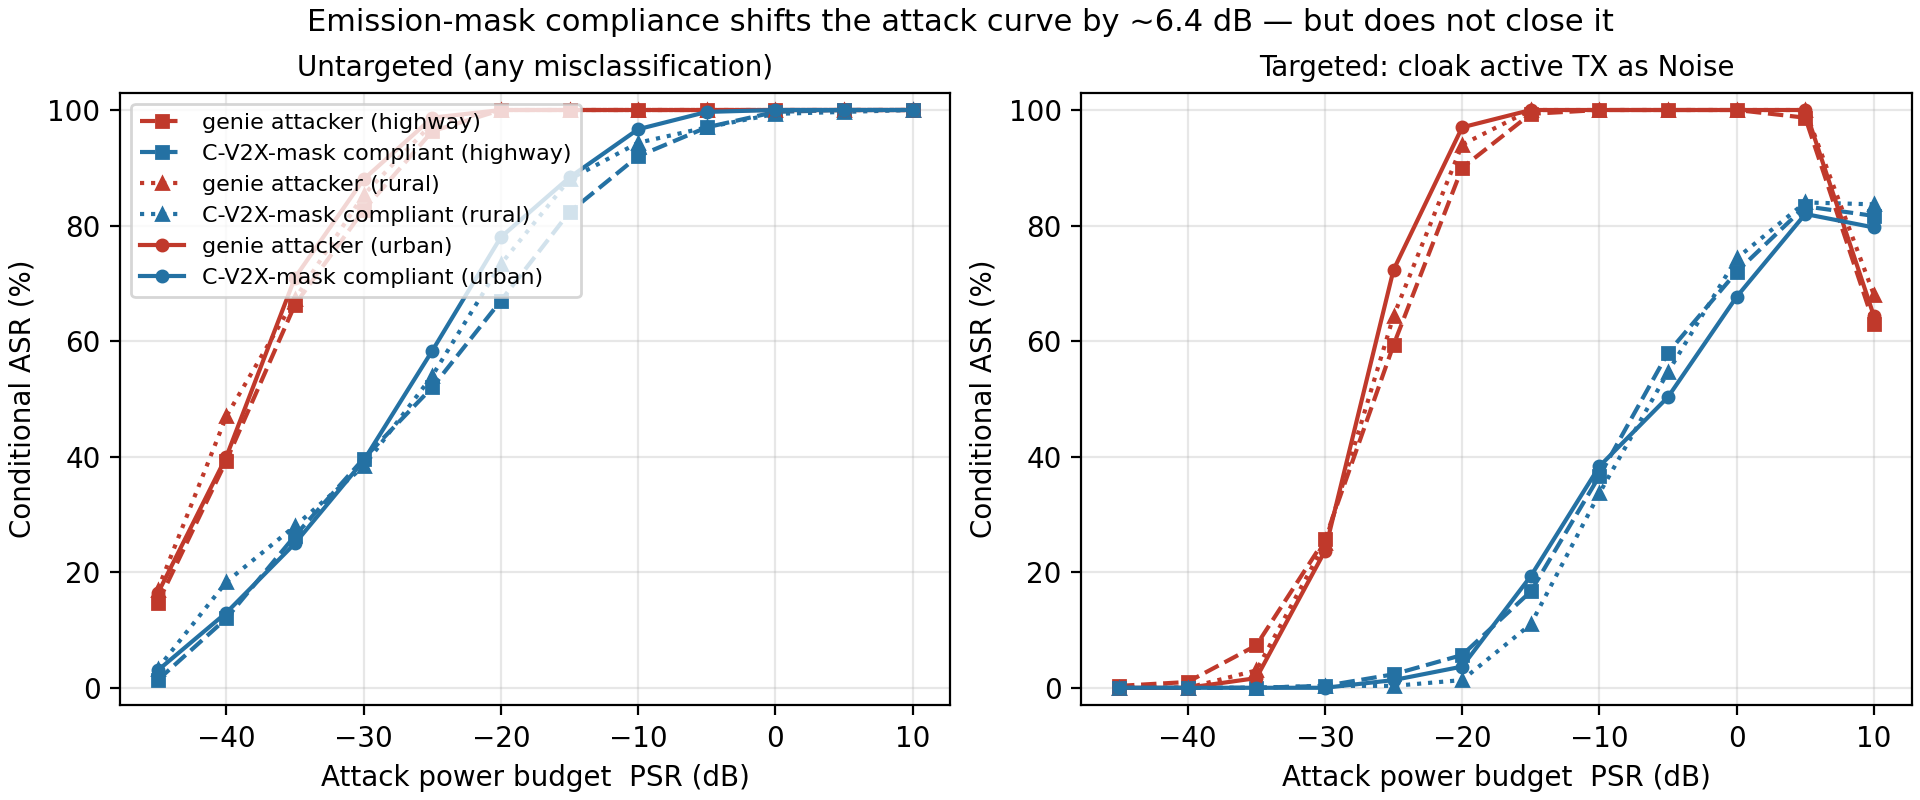
\includegraphics[width=0.95\linewidth]{figs/price_of_compliance.png}
\caption{Conditional ASR versus attack power budget (PSR, dB) for genie vs
emission-mask-compliant attackers, untargeted and targeted-to-Noise modes,
urban, highway, and rural channels (prototype protocol of
Table~\ref{tab:protocol}). Compliance shifts the attack curve right by
${\sim}$5--7\,dB (untargeted) but does not close it; both attackers break the
undefended CNN at deeply negative PSR.}
\label{fig:poc}
\end{figure}

\begin{table}[t]
\centering
\caption{Physical summary metrics (conditional-ASR threshold 20\%;
prototype protocol of Table~\ref{tab:protocol}; all MEAPs resolved within
the grid, no censoring).}
\label{tab:metrics}
\begin{tabular}{llrrr}
\toprule
Scenario & Mode & MEAP genie & MEAP compliant & Price of Compliance \\
\midrule
urban & untargeted & $-44.2$ dB & $-37.1$ dB & $7.1$ dB \\
highway & untargeted & $-43.9$ dB & $-37.2$ dB & $6.7$ dB \\
rural & untargeted & $-44.5$ dB & $-39.1$ dB & $5.4$ dB \\
urban & targeted-noise & $-30.8$ dB & $-14.8$ dB & $16.0$ dB \\
highway & targeted-noise & $-31.5$ dB & $-14.2$ dB & $17.4$ dB \\
rural & targeted-noise & $-31.1$ dB & $-13.0$ dB & $18.1$ dB \\
\bottomrule
\end{tabular}
\end{table}

Four findings emerge (Fig.~\ref{fig:poc}, Table~\ref{tab:metrics}).
\textbf{(F1) Undefended CNNs are catastrophically
brittle in absolute terms.} The genie attacker reaches 20\% conditional ASR
at $-44$\,dB---four orders of magnitude below the received signal---and the
\emph{compliant} attacker at $-37$\,dB. At $-10$\,dB (an attacker ten times
weaker than the victim signal), the compliant attacker achieves 96.7\%
(urban) / 92.0\% (highway) conditional ASR, and 39.3\% (urban) /
39.7\% (highway) even at $-30$\,dB. \textbf{(F2) Compliance costs
${\sim}$5--7\,dB} for generic misclassification, consistently across urban,
highway, and rural channels---the price is a property of the mask, not the
channel. \textbf{(F3) Cloaking is the costlier attack:} forcing the specific
``Noise'' label costs the compliant attacker 16--18\,dB more than the genie
(0.4\% or less conditional ASR below $-25$\,dB; 38.3\%/36.7\% at
$-10$\,dB; 68\%/72\% at parity).
Target specificity, not generic misclassification, is where the mask bites.
\textbf{(F4) Overshoot at high power:} at $+10$\,dB the targeted attack's
Noise-specific success \emph{decreases} (genie 63--68\%, compliant
80--84\%) while untargeted damage saturates---the perturbation overshoots
into other wrong classes (robust accuracy is 8--14\%), a real phenomenon for certified-decision pipelines
that key on specific labels.

\paragraph{Robustness of the metrics} Three checks bound the main threats to
validity of Table~\ref{tab:metrics}. \emph{Attack-strength convergence:}
PGD-50 (versus PGD-10) shifts the compliant MEAP by only $-1.7$\,dB (to
$-38.8$\,dB; its genie MEAP is censored at that grid's floor) and raises
mid-grid conditional ASR substantially (up to $+37$\,pp at $-25$\,dB)---the
zero-initialized, restart-free PGD-10 protocol therefore reports materially
\emph{conservative} attack numbers, and the PGD-10 MEAPs are lower bounds.
\emph{Seed stability:} a second attack
seed (11) reproduces the urban untargeted PoC at 6.9\,dB versus 7.1\,dB
(0.3\,dB spread; MEAPs move by $\le$1\,dB). \emph{Mask-cap idealization:}
relaxing the flat in-band cap from $2\times$ to $10\times$ uniform sharing
moves the compliant MEAP by only $-0.9$\,dB and the PoC from 7.1 to
6.2\,dB---the Price of Compliance is driven by the \emph{allocation}
constraint (the out-of-band null), not by how strictly in-band flatness is
enforced. \emph{Attacker knowledge:} re-running the compliant attack with
imperfect CSI (additive error of 0.3 relative magnitude) costs only
1--2\,pp of conditional ASR across the grid (MEAP within 0.5\,dB)---the
attack is robust to CSI error; but with \emph{no} CSI (optimizing against
an independent draw from the same scenario, evaluated on the true channel)
the compliant attack's 20\%\,ASR threshold moves from $-37$\,dB to
$\approx\!-16$\,dB, a $\sim$21\,dB penalty: channel-realization
knowledge, not channel statistics, is what makes the white-box threat
catastrophic. \FULLP{Three-seed training error bars complete the statistics at
full scale.}

\subsection{What the legacy feature-space threat model silently assumes}
\label{sec:featurespace}

A log-magnitude perturbation of $\pm\epsilon$ (in z-scored units) in the
receiver's spectrogram has no direct physical meaning. It can be given one:
a log-magnitude change $d$ on bin $k$ corresponds to the complex STFT-domain
addition $\hat{\Delta}_k = \hat{Z}_k (10^{d} - 1)$ (magnitude scaling, phase
preserved), and the hann/50\%-overlap STFT is invertible (interior
reconstruction error $< 10^{-5}$), so the same edit implies a
\emph{received} waveform perturbation whose power we can measure
(PSR$_{\mathrm{eq}}$). We attack the magnitude input with an
$\ell_\infty$ PGD ($\epsilon \in \{0.1, 0.3, 1.0\}$) and translate the
perturbation to the waveform domain. At $\epsilon = 1.0$ (one standard
deviation of the log-magnitude distribution) the feature-space attack
achieves 71.3\% conditional ASR \emph{as evaluated in the legacy setting}
(the perturbed spectrogram is fed directly to the CNN), while its implied
received power is $-24$\,dB (median). Feeding the actual waveform
$x + \delta_{\mathrm{rx}}$ through the receiver's true front-end realizes
only 14.0\%: the hann-window round trip realizes roughly half of the
intended per-bin log-change, and the receiver noise absorbs the rest. By
contrast, \emph{transmitted} attacks optimized for that same power
($-24$\,dB) achieve 99.3\% (genie) and 62.3\% (compliant). At
$\epsilon \le 0.3$ the legacy attack achieves essentially nothing (0--1.7\%)
at implied powers of $-34$ to $-44$\,dB. Three lessons: (i) the
feature-space $\epsilon$-ball hides a power budget that is invisible in
$\epsilon$-units; (ii) a feature-space perturbation is not a physically
consistent waveform---its own physical realization mostly fails, so legacy
feature-space ASRs overstate realizable attacks at the implied power;
(iii) an adversary that can actually transmit is far better served by
optimizing the waveform directly (as in this paper) than by hoping an
$\epsilon$-ball transfers. Comparisons of ASR across threat models are
meaningless without the PSR$_{\mathrm{eq}}$ translation.

\subsection{Defenses: mask-matched adversarial training}
\label{sec:defenses}

The natural defense is adversarial training inside the same feasible set:
during training, each minibatch is (with probability 0.5) adversarially
perturbed by a 5-step mask-compliant waveform PGD attack at a PSR drawn
uniformly from $[-25, -5]$\,dB, with a fresh attacker channel, generated
against the current model and added through that channel; training otherwise
follows the standard recipe. The defended model retains \emph{100\%} clean
validation accuracy. Against the identical attack protocol (urban,
untargeted, seed 7, PGD-10): the genie MEAP shifts from $-44.2$ to
$-37.5$\,dB ($+6.8$\,dB), the \emph{compliant} MEAP from $-37.1$ to
$-23.1$\,dB ($+14.0$\,dB), and the Price of Compliance doubles from 7.1 to
14.4\,dB. Point-wise, the compliant attacker's conditional ASR at $-25$\,dB
collapses from 58.3\% to 16.7\%, and at $-10$\,dB from 96.7\% to 55.3\%;
targeted cloaking at $-10$\,dB falls from 38.3\% to 15.0\%. Compliance and
adversarial training thus compound: each buys roughly 7--8\,dB
independently, and together they push the compliant attacker's
20\%-ASR threshold from $-37$\,dB to $-23$\,dB. The defense has an honest
boundary: robustness is confined to the trained power range---at PSR parity
and above the attack still succeeds (94.7\% at 0\,dB), and attacks far below
the training range partially transfer. Adversarial training \emph{delays} the
attack exactly as compliance does; neither closes it, and the
certification-style metric (MEAP) is what quantifies both. \FULLP{A
TRADES-style trade-off variant and statistical detection~\cite{zhao2024} as
a complementary control are evaluated at full scale.}

\section{Standards, Deployment Implications, and Ethics}
\label{sec:standards}

The compliant-attacker threat model is deliberately aligned with how
spectrum rules are enforced, which makes the results actionable in the
O-RAN and conformance-testing contexts mapped by adversarial-ML threat
analyses~\cite{habler2025}. Five deployment scenarios, stated with their
preconditions and non-claims:

\begin{itemize}
\item \textbf{O-RAN RIC robustness gate:} security engineers run the
released compliant-attack suite against ML-based sensing xApps before
deployment, requiring MEAP above a policy margin; conditional-ASR and PoC
are logged as security KPIs. Single-receiver, differentiable-model scope; no
network-level guarantees.
\item \textbf{FCC transition margin budgeting:} during the 5.9\,GHz
transition~\cite{fcc2020,fcc2024}, vendors and regulators use the
compliant-ASR-vs-PSR curves as worst-case inputs when setting sensing
thresholds and guard strategies for coexistence receivers. Not field
measurements; non-compliant jammers are out of scope.
\item \textbf{ETSI-style conformance extension:} conformance labs replay
standardized mask-compliant adversarial waveforms through channel emulators
into devices under test, complementing EN~302~571 unwanted-emission and
blocking tests~\cite{etsi302571} with receiver-side adversarial robustness
reporting. Not an established test case; not a substitute for OTA.
\item \textbf{Benchmark for the sub-niche:} the released generators,
channels, attack, and metrics with embedded configurations give
attack/defense papers a common substrate---today every paper self-defines
its threat model, blocking comparison.
\item \textbf{Vendor CI regression gate:} ML teams run the mask-constrained
attack nightly on frozen evaluation sets, alerting when MEAP drops or
compliant ASR rises beyond tolerance, catching silent robustness
regressions across model releases. Requires differentiable model export;
minutes of CPU per run at prototype scale.
\end{itemize}

\paragraph{Responsible disclosure} The attack operates within existing
regulatory power limits and cannot create spectrum violations; the released
code enables defensive evaluation, and the defense section quantifies
mitigation. We release all artifacts so that the threat model can be
audited, extended, and defended against---the standard rationale for
adversarial-ML publications.

\section{Limitations}
\label{sec:limitations}

(1)~Waveforms are synthetic and standard-parameterized, not OTA captures;
pilots, preambles, and higher-order modulations are not modeled.
(2)~The emission mask is idealized: a flat in-band cap (stricter than real
in-band rules, which permit PRB-level concentration) and a hard OOB null;
the $2\times\!\to\!10\times$ cap relaxation shifts the PoC by only
$-0.9$\,dB, so the allocation constraint dominates; a PRB-granular in-band
model remains future work.
(3)~Channels are TR~37.885-inspired simplifications (first-tap-only Rician,
UMa-flavored urban spread), block-fading within the window---defensible by
Doppler coherence, but approximate.
(4)~The prototype attacker is white-box with perfect CSI and exact knowledge
of the received realization (worst-case upper bound; the CSI-mismatch
variant is released); PGD is zero-initialized without restarts, making
reported ASRs lower bounds on the attack side and upper bounds on the
defense side.
(5)~Prototype scale: one training seed, two attack seeds, 300 windows,
PGD-10 (PGD-50 and seed stability checked on key conditions: shifts
$\le$1.7\,dB); \FULLP{the full 3-seed protocol completes the statistics}.
(6)~The phase-difference stream contributes nothing on this task; the
``phase-aware'' framing of our prior work is retired honestly.
(7)~The adversarially-trained defense's robustness is confined to its
training power range ($-25$ to $-5$\,dB); attacks at parity or above still
succeed, and a TRADES-style trade-off study is deferred.

\section{Conclusion}
\label{sec:conclusion}

Emission-mask compliance is not a defense: it shifts the adversarial attack
curve on DL ITS-band spectrum sensing by only ${\sim}$5--7\,dB (untargeted)
and 16--18\,dB (targeted cloaking), while an undefended CNN is broken by a
rule-abiding transmitter operating tens of dB below the victim signal. The
legacy feature-space threat model, translated to physical power, overstates
realizable attacks: its own perturbation, made physical, mostly fails, while
a purpose-optimized waveform at the same implied power is far stronger; the
PSR-equivalence translation makes such comparisons meaningful. The compliant-attacker threat
model, the MEAP and Price-of-Compliance metrics, and the released
end-to-end framework give regulators, standards bodies, and O-RAN security
engineers a physically grounded, certification-ready way to measure---and,
with mask-matched adversarial training (+14\,dB at zero clean-accuracy
cost), to raise---the cost of attacking deep-learning spectrum sensing.

% ============================================================================
\begin{thebibliography}{99}

\bibitem{o2018} T. J. O'Shea, T. Roy, T. C. Clancy,
``Over-the-air deep learning based radio signal classification,''
\emph{IEEE J. Sel. Topics Signal Process.}, vol. 12, no. 1, pp. 168--179,
Feb. 2018, doi: 10.1109/JSTSP.2018.2797022.

\bibitem{girmay2023} M. Girmay, V. Maglogiannis, D. Naudts, M. Aslam,
A. Shahid, I. Moerman, ``Technology recognition and traffic characterization
for wireless technologies in ITS band,'' \emph{Vehicular Communications},
vol. 39, art. 100563, Feb. 2023, doi: 10.1016/j.vehcom.2022.100563.

\bibitem{sadeghi2019} M. Sadeghi, E. G. Larsson, ``Adversarial attacks on
deep-learning based radio signal classification,'' \emph{IEEE Wireless
Commun. Lett.}, vol. 8, no. 1, pp. 213--216, Feb. 2019,
doi: 10.1109/LWC.2018.2867459.

\bibitem{kim2020} B. Kim, Y. E. Sagduyu, K. Davaslioglu, T. Erpek,
S. Ulukus, ``Over-the-air adversarial attacks on deep learning based
modulation classifier over wireless channels,'' in \emph{Proc. 54th Annu.
Conf. Information Sciences and Systems (CISS)}, 2020, pp. 1--6,
doi: 10.1109/CISS48834.2020.1570617416.

\bibitem{sagduyu2021} B. Kim, Y. E. Sagduyu, K. Davaslioglu, T. Erpek,
S. Ulukus, ``Channel-aware adversarial attacks against deep learning-based
wireless signal classifiers,'' \emph{IEEE Trans. Wireless Commun.}, vol. 21,
no. 6, pp. 3868--3880, Jun. 2022, doi: 10.1109/TWC.2021.3124855.

\bibitem{liu2022} M. Liu, H. Zhang, Z. Liu, N. Zhao, ``Attacking spectrum
sensing with adversarial deep learning in cognitive radio-enabled Internet of
Things,'' \emph{IEEE Trans. Rel.}, vol. 72, no. 2, pp. 431--444, Jun.
2023, doi: 10.1109/TR.2022.3179491.

\bibitem{zheng2026} S. Zheng, Z. Ye, L. Zhang, K. Yue, Z. Zhao, ``Targeted
adversarial attacks against deep learning-based wideband spectrum sensing,''
\emph{IEEE Trans. Mach. Learn. Commun. Netw.}, vol. 4, pp. 950--965, 2026,
doi: 10.1109/TMLCN.2026.3694666.

\bibitem{radioshock2026} W. Li, C. Li, G. Zhang, Z. Huang, G. Qu, X. Cheng,
J. Luo, P. Hu, ``RadioShock: over-the-air adversarial attacks on wireless
communication,'' \emph{IEEE Trans. Dependable Secur. Comput.}, vol. 23,
no. 4, pp. 8874--8890, 2026, doi: 10.1109/TDSC.2026.3689592.

\bibitem{zhao2024} W. Zhao, X. Li, S. Zhao, J. Xu, Y. Liu, Z. Lu,
``Detecting adversarial spectrum attacks via distance to decision boundary
statistics,'' in \emph{Proc. IEEE INFOCOM}, 2024, pp. 691--700,
doi: 10.1109/INFOCOM52122.2024.10621153.

\bibitem{croce2020} F. Croce, M. Hein, ``Reliable evaluation of adversarial
robustness with an ensemble of diverse parameter-free attacks,'' in
\emph{Proc. 37th Int. Conf. Machine Learning (ICML)}, PMLR, vol. 119, 2020,
pp. 2206--2216.

\bibitem{habler2025} E. Habler, R. Bitton, D. Avraham, E. Klevansky,
D. Mimran, O. Brodt, H. Lehmann, Y. Elovici, A. Shabtai, ``Adversarial
machine learning threat analysis and remediation in Open Radio Access
Network (O-RAN),'' \emph{J. Netw. Comput. Appl.}, vol. 236, art. 104090,
Apr. 2025, doi: 10.1016/j.jnca.2024.104090.

\bibitem{fcc2020} Federal Communications Commission, ``Use of the
5.850--5.925~GHz Band,'' First Report and Order, FCC 20-164, ET Docket
No. 19-138, adopted Nov. 18, 2020 (published at 86 FR 23281, May 3, 2021).

\bibitem{fcc2024} Federal Communications Commission, ``Use of the
5.850--5.925~GHz Band,'' Second Report and Order, FCC 24-123, ET Docket
No. 19-138, adopted Nov. 20, 2024 (published at 89 FR 100838, Dec. 13,
2024; effective Feb. 11, 2025).

\bibitem{etsi302571} ETSI, ``Intelligent Transport Systems (ITS);
Radiocommunications equipment operating in the 5~855~MHz to 5~925~MHz
frequency band; Harmonised Standard covering the essential requirements of
article 3.2 of Directive 2014/53/EU,'' ETSI EN 302 571, V2.1.1, Feb. 2017.

\bibitem{tr37885} 3GPP, ``Study on evaluation methodology of new
Vehicle-to-Everything (V2X) use cases for LTE and NR,'' 3GPP TR 37.885,
V15.3.0, Release 15, Jun. 2019.

\bibitem{ts36211} 3GPP, ``Evolved Universal Terrestrial Radio Access
(E-UTRA); Physical channels and modulation,'' 3GPP TS 36.211, V15.14.0,
Release 15, Oct. 2021.

\bibitem{ieee80211} IEEE, ``IEEE Standard for Information
technology---Telecommunications and information exchange between
systems---Local and metropolitan area networks---Specific
requirements---Part 11: Wireless LAN Medium Access Control (MAC) and
Physical Layer (PHY) Specifications,'' IEEE Std 802.11-2012, 2012.

\bibitem{dhankhar2026} P. Dhankhar, D. Vats, ``Dual-stream phase-aware
Inception-Time CNN for adversarially robust spectrum sensing in V2X
networks,'' in \emph{Proc. Int. Conf. Computing, Communication, and
Technologies (ICE2CT)}, 2026.

\end{thebibliography}

\end{document}
